%%
%% CausalLens: An Open-Source Toolkit for Causal Autonomy Auditing
%% of Recommender Systems
%%
%% ACM RecSys 2026  —  acmart sigconf
%%

\documentclass[sigconf,nonacm=false]{acmart}

%% ── packages ────────────────────────────────────────────────────────
\usepackage{booktabs}
\usepackage{graphicx}
\usepackage{subcaption}

%% ── paths ───────────────────────────────────────────────────────────
\graphicspath{{../results/figures/}}

%% ── theorem-like environments ───────────────────────────────────────
\newtheorem{definition}{Definition}

%% ── metadata ────────────────────────────────────────────────────────
\title{CausalLens: An Open-Source Toolkit for Causal Autonomy Auditing of Recommender Systems}

\author{Stefano Casafranca}
\affiliation{%
  \institution{University of Calgary}
  \city{Calgary}
  \state{Alberta}
  \country{Canada}
}
\email{stefano.casafranca@ucalgary.ca}

\begin{abstract}
Observational metrics such as intra-list diversity and recommendation volatility are widely used to assess whether recommender systems respect user autonomy. We show these metrics systematically fail: across 800 user evaluations spanning two architectures and two datasets, 68--94\% of users who \emph{appear} autonomous by observational criteria are in fact causally trapped---their recommendations cannot be meaningfully altered by their own actions, yet can be shifted by adversarial manipulation of other users' ratings. We introduce \textbf{CausalLens}, an open-source Python toolkit that operationalizes the causal autonomy auditing framework of Sharma et al.\ (2024) into four computable metrics: Reachability Cost, Manipulation Resistance, Autonomy Asymmetry Index (AAI), and Observational Deception Rate (ODR). CausalLens provides both white-box gradient-based and black-box query-based computation paths, supports any recommender exposing a predict/update interface, and reproduces our full experimental pipeline on a single laptop. Our ablation across Matrix Factorization and Neural Collaborative Filtering reveals that cross-user parameter sharing in neural architectures amplifies manipulation vulnerability by 25.4\% while inflating ODR from 68.3\% to 90.4\% on MovieLens-1M. Code and data are publicly available at \url{https://github.com/stefanocasafranca/CausalLens}.
\end{abstract}

\begin{CCSXML}
<ccs2012>
   <concept>
       <concept_id>10002951.10003317.10003347.10003350</concept_id>
       <concept_desc>Information systems~Recommender systems</concept_desc>
       <concept_significance>500</concept_significance>
   </concept>
   <concept>
       <concept_id>10002951.10003317.10003371</concept_id>
       <concept_desc>Information systems~Evaluation of retrieval results</concept_desc>
       <concept_significance>300</concept_significance>
   </concept>
</ccs2012>
\end{CCSXML}

\ccsdesc[500]{Information systems~Recommender systems}
\ccsdesc[300]{Information systems~Evaluation of retrieval results}

\keywords{recommender systems, causal auditing, user autonomy, manipulation resistance, observational deception}

\begin{document}

\maketitle

%% ═════════════════════════════════════════════════════════════════════
\section{Introduction}
\label{sec:intro}
%% ═════════════════════════════════════════════════════════════════════

In 2024, a user reported that after a friend engaged with cocaine-related content on Instagram, drug-related recommendations began appearing in \emph{their own} feed---despite never interacting with such content themselves. No tool existed to measure this cross-user influence, quantify its magnitude, or determine whether the affected user could escape it through their own actions.

This incident illustrates a fundamental limitation of current recommender system auditing. Regulators and researchers rely on \emph{observational} metrics---diversity of recommended items, catalog coverage, recommendation volatility---to assess whether systems respect user autonomy~\cite{eu_dsa2022, ge2010beyond, zhang2008avoiding}. These metrics capture surface-level properties of recommendation lists but cannot distinguish between a user who genuinely controls their feed and one whose apparent autonomy is an artifact of the system's internal dynamics.

Sharma et al.~\cite{sharma2024unified} formalized this distinction through a causal framework for auditing recommender systems, defining metrics grounded in interventional reasoning: what happens when a user \emph{tries} to change their recommendations, and what happens when an adversary \emph{tries} to change them for someone else. Their framework provides the theoretical foundation, but no reproducible implementation exists.

\textbf{CausalLens} fills this gap. We contribute:
\begin{enumerate}
    \item An \textbf{open-source toolkit} operationalizing four causal autonomy metrics with both white-box and black-box computation paths;
    \item \textbf{Reachability Cost} and \textbf{Manipulation Resistance} formulated as constrained optimization problems with gradient-based and query-based solvers;
    \item Two novel composite metrics---\textbf{Autonomy Asymmetry Index} (AAI) and \textbf{Observational Deception Rate} (ODR)---that directly quantify the gap between observational and causal assessments;
    \item The \textbf{first empirical ablation} of causal vs.\ observational auditing methods across architectures (MF vs.\ NeuMF) and datasets (MovieLens-1M vs.\ Amazon Musical Instruments), revealing that 68--94\% of observationally autonomous users are causally trapped.
\end{enumerate}


%% ═════════════════════════════════════════════════════════════════════
\section{Related Work}
\label{sec:related}
%% ═════════════════════════════════════════════════════════════════════

\paragraph{Causal auditing theory.}
Sharma et al.~\cite{sharma2024unified} proposed a unified causal framework for auditing recommender systems, formalizing notions of reachability, manipulation, and autonomy using Pearl's causal inference machinery~\cite{pearl2009causality}. Their work establishes the theoretical foundations we operationalize. CausalLens translates their definitions into computable algorithms with both gradient-based (white-box) and query-based (black-box) solvers, and conducts the first large-scale empirical evaluation of causal vs.\ observational auditing.

\paragraph{Reachability in recommender systems.}
Dean et al.~\cite{dean2020recommendations} introduced the concept of reachability in collaborative filtering, asking whether users can reach arbitrary items through rating changes. Curmei et al.~\cite{curmei2021towards} extended this with psychologically-grounded preference dynamics. CausalLens builds on these foundations by (i) coupling reachability with adversarial manipulation resistance into a unified audit, and (ii) introducing the ODR metric that exposes the gap between observational and causal assessments.

\paragraph{Steerability evaluation.}
SteerEval~\cite{steereval2026} measures the steerability of natural language-profile recommender systems. While conceptually related, its scope is narrower: it targets a single system type (NL-profile recommenders), does not measure cross-user manipulation resistance, and does not provide a general-purpose toolkit.

\paragraph{Regulatory auditing.}
``Beyond the Checkbox''~\cite{beyondcheckbox2026} analyzed the first Digital Services Act audit reports from YouTube, Instagram, and TikTok, finding significant methodological gaps in how platforms assess algorithmic influence. ``Rethinking User Empowerment''~\cite{rethinkingempowerment2026} proposed design provotypes for user agency but focuses on interface design rather than quantitative measurement. Both works demonstrate the regulatory need that CausalLens addresses with concrete tooling.

\paragraph{Observational metrics.}
Intra-list diversity~\cite{zhang2008avoiding}, catalog coverage~\cite{ge2010beyond}, and recommendation volatility are standard beyond-accuracy metrics. Our ODR metric demonstrates that these observational indicators can be systematically misleading when used as proxies for user autonomy.


%% ═════════════════════════════════════════════════════════════════════
\section{Formal Definitions}
\label{sec:definitions}
%% ═════════════════════════════════════════════════════════════════════

Let $\mathcal{U} = \{1, \ldots, n\}$ be the set of users, $\mathcal{V} = \{1, \ldots, m\}$ the set of items, $\mathbf{r}_i \in \mathbb{R}^m$ user $i$'s rating vector, $R \in \mathbb{R}^{n \times m}$ the full rating matrix, $f$ the recommender function, $\text{top-}k(f, i)$ the set of $k$ recommended items for user $i$, and $d(\cdot, \cdot)$ the Jaccard distance between two top-$k$ sets.

\begin{definition}[Reachability Cost]
\label{def:reachability}
The reachability cost for user $i$ to reach item $j$ in the top-$k$ is:
\begin{equation}
    \mathcal{R}(i, j, k) = \min_{\delta} \|\delta\|_1 \quad \text{s.t.} \quad \text{rank}(f, j, i \mid \mathbf{r}_i + \delta) \leq k, \; \delta \in \mathcal{C}
\end{equation}
where $\mathcal{C}$ constrains perturbations to valid rating values applied to user $i$'s \emph{own} ratings.
\end{definition}

\noindent \textbf{Intuition.} Reachability cost measures how many of their own ratings a user must change to push a target item into their top-$k$. High cost means the user is ``stuck''---unable to meaningfully steer their recommendations.

\begin{definition}[Manipulation Resistance]
\label{def:manipulation}
The manipulation resistance of user $i$ against adversary $a$ with budget $\varepsilon$ is:
\begin{equation}
    \mathcal{M}(i, a, \varepsilon) = \max_{\delta_a} d\!\left(\text{top-}k(f, i \mid R), \; \text{top-}k(f, i \mid R + \Delta_a)\right) \quad \text{s.t.} \quad \|\delta_a\|_1 \leq \varepsilon
\end{equation}
where $\Delta_a$ modifies \emph{only} adversary $a$'s ratings.
\end{definition}

\noindent \textbf{Intuition.} Manipulation resistance quantifies how much a stranger can shift a victim's recommendations by changing only their own ratings. Low resistance (high displacement) means the user's feed is vulnerable to cross-user influence.

\begin{definition}[Autonomy Asymmetry Index]
\label{def:aai}
Let $S(i, \varepsilon) = d(\text{top-}k(f, i \mid R), \text{top-}k(f, i \mid R + \Delta_i^*))$ be the self-influence displacement (maximum shift from the user's own budget-$\varepsilon$ perturbation), and $E(i, \varepsilon) = \max_a \mathcal{M}(i, a, \varepsilon)$ the maximum adversary displacement. The Autonomy Asymmetry Index is:
\begin{equation}
    \text{AAI}(i, \varepsilon) = \frac{E(i, \varepsilon)}{S(i, \varepsilon)}
\end{equation}
\end{definition}

\noindent \textbf{Intuition.} AAI $< 1$ means the user has more influence over their own feed than any adversary (healthy). AAI $> 1$ means an external actor can move the user's recommendations more than the user themselves can (problematic).

\begin{definition}[Observational Deception Rate]
\label{def:odr}
Let $\mathcal{A} \subset \mathcal{U}$ be the set of users flagged as autonomous by observational criteria (diversity above median \emph{and} volatility above median, computed within each model--dataset combination). Let $\mathcal{T} \subset \mathcal{U}$ be users who are causally trapped (reachability success rate $= 0$). The Observational Deception Rate is:
\begin{equation}
    \text{ODR} = \frac{|\mathcal{A} \cap \mathcal{T}|}{|\mathcal{A}|}
\end{equation}
\end{definition}

\noindent \textbf{Intuition.} ODR measures the fraction of users who \emph{look} autonomous by standard metrics but are in fact unable to change their recommendations through their own actions. High ODR means observational auditing systematically fails to detect causal entrapment.


%% ═════════════════════════════════════════════════════════════════════
\section{System Design}
\label{sec:system}
%% ═════════════════════════════════════════════════════════════════════

CausalLens is a Python library structured around an abstract \texttt{Recommender} interface that any model can implement by exposing three methods: \texttt{get\_scores(user, R)} for raw score computation, \texttt{get\_recommendations(user, R, k)} for top-$k$ retrieval, and \texttt{fit(R)} for training. This abstraction enables CausalLens to audit arbitrary recommender architectures without modification to the underlying model code.

\paragraph{Computation paths.}
CausalLens provides two computation paths for each metric:
\begin{itemize}
    \item \textbf{White-box (gradient-based):} For differentiable models (MF, NeuMF), reachability uses two-phase projected gradient descent---first maximizing the target item's score, then binary-searching the minimum budget. Manipulation resistance uses gradient ascent on the adversary's ratings to maximize Jaccard displacement. The MF scoring path uses a differentiable soft-sigmoid weighted ridge regression: $w_j = \sigma((r_j - 0.5) \cdot 20)$, ensuring unrated items receive near-zero weight while perturbations smoothly introduce new ratings.
    \item \textbf{Black-box (query-based):} For non-differentiable or API-only models, reachability uses greedy coordinate search (in-place modify/restore, avoiding matrix copies), and manipulation resistance uses hill-climbing with random restarts.
\end{itemize}

\paragraph{Cross-user coupling.}
For models with shared parameters (NeuMF), adversary perturbations trigger a warm-start retrain of shared item embeddings, propagating effects to all users' scores. NeuMF uses step-limited retraining (50 SGD steps) for practical black-box search, with a cached scratch model for fast user fine-tuning.

\paragraph{Pipeline.}
The end-to-end audit pipeline: load data $\rightarrow$ train model $\rightarrow$ select users $\rightarrow$ compute per-user metrics (reachability, manipulation, AAI, observational baselines) $\rightarrow$ compute ODR $\rightarrow$ aggregate and report. The full experiment reproduces on a single laptop via \texttt{python run\_all.py}.


%% ═════════════════════════════════════════════════════════════════════
\section{Experiments}
\label{sec:experiments}
%% ═════════════════════════════════════════════════════════════════════

\paragraph{Models.}
We evaluate two architectures implemented from scratch within CausalLens:
\begin{itemize}
    \item \textbf{Matrix Factorization (MF)}~\cite{koren2009matrix}: 64-dimensional user/item factors trained with SGD for 20 epochs (batch size 1024). MF with frozen item factors isolates user-specific effects---each user's scores depend only on their own ratings, providing a baseline with no cross-user coupling.
    \item \textbf{Neural Collaborative Filtering (NeuMF)}~\cite{he2017neural}: GMF (32-dim) + MLP (64$\to$32$\to$16) dual-path architecture, 15 epochs, batch size 1024. NeuMF shares item embeddings across users; adversary perturbations trigger 25-step warm-start retrains of shared parameters, creating measurable cross-user coupling.
\end{itemize}

\paragraph{Datasets.}
\begin{itemize}
    \item \textbf{MovieLens-1M}~\cite{harper2015movielens}: 6,040 users, 3,706 items, 1M explicit ratings (1--5).
    \item \textbf{Amazon Musical Instruments}~\cite{mcauley2015image}: 5-core subset with explicit ratings from the Amazon Reviews 2023 corpus.
\end{itemize}

\paragraph{Protocol.}
For each of the four model--dataset combinations, we sample 200 users with $\geq 20$ ratings ($N = 800$ total evaluations). Per user: 5 reachability targets (random unrated items outside current top-$k$) with budget $B = 20$ rating changes and 50 gradient steps (MF) or 20 random-search trials (NeuMF); 3 random adversaries with budget $\varepsilon = 5$; self-influence with budget $\varepsilon = 5$. Observational autonomy thresholds are set at within-combo medians of diversity and volatility. All experiments use $k = 10$ and Jaccard distance.

\paragraph{Budget justification.}
The reachability budget $B = 20$ reflects a conservative estimate of realistic attacker constraints---a user or adversary altering more than 20 ratings represents a substantial behavioral change. As we show in Section~\ref{sec:results}, this stringent budget means most target items remain unreachable, which is itself an informative finding about the structural rigidity of recommendation paths.


%% ═════════════════════════════════════════════════════════════════════
\section{Results}
\label{sec:results}
%% ═════════════════════════════════════════════════════════════════════

\begin{table}[t]
\centering
\small
\resizebox{\columnwidth}{!}{%
\begin{tabular}{lrcccr}
\toprule
Model / Dataset & $N$ & Reach.\ cost & Manip.\ disp. & AAI & ODR (\%) \\
 & & (mean $\pm$ std) & (mean $\pm$ std) & (mean $\pm$ std) & \\
\midrule
MF / ML-1M & 200 & $19.25 \pm 1.73$ & $0.453 \pm 0.143$ & $0.785 \pm 0.430$ & 68.3 \\
NeuMF / ML-1M & 200 & $7.89 \pm 5.16$ & $0.518 \pm 0.117$ & $0.733 \pm 0.161$ & 90.4 \\
MF / Amazon-MI & 200 & $18.46 \pm 3.10$ & $0.576 \pm 0.137$ & $0.681 \pm 0.157$ & 88.0 \\
NeuMF / Amazon-MI & 200 & $10.33 \pm 5.89$ & $0.772 \pm 0.102$ & $0.841 \pm 0.095$ & 93.9 \\
\bottomrule
\end{tabular}}
\caption{Main results across architectures and datasets. NeuMF exhibits substantially higher manipulation displacement than MF, confirming cross-user coupling through shared neural embeddings. Reachability cost is reported over finite-cost users only (users with no target reached within budget are excluded from the mean). ODR denominators (observationally autonomous users): MF / ML-1M 28/41, NeuMF / ML-1M 47/52, MF / Amazon-MI 44/50, NeuMF / Amazon-MI 46/49.}
\label{tab:main-results}
\end{table}

\begin{table}[t]
\centering
\small
\resizebox{\columnwidth}{!}{%
\begin{tabular}{lcccr}
\toprule
Model / Dataset & ILD (mean) & Coverage & Volatility (mean) & ODR (\%) \\
\midrule
MF / ML-1M & 0.733 & 0.096 & 0.125 & 95.1 \\
NeuMF / ML-1M & 0.837 & 0.102 & 0.576 & 89.3 \\
LightGCN / ML-1M & 0.607 & --- & 0.000 & 0.0 \\
SASRec / ML-1M & 0.918 & --- & 0.055 & 14.3 \\
MF / Amazon-MI & 0.983 & 0.017 & 0.357 & 94.5 \\
NeuMF / Amazon-MI & 0.999 & 0.044 & 0.721 & 94.3 \\
LightGCN / Amazon-MI & 1.000 & --- & 0.054 & 0.0 \\
SASRec / Amazon-MI & 0.999 & --- & 0.050 & 0.0 \\
\bottomrule
\end{tabular}}
\caption{Observational baselines and ODR per combination. ILD and volatility are per-user means; catalog coverage is population-level. ODR is the fraction of users flagged observationally autonomous (diversity ${>}$ median AND volatility ${>}$ median, within combo) who fail the causal reachability test (zero successes).}
\label{tab:odr-breakdown}
\end{table}


\subsection{Observational Deception Is Pervasive}

The headline finding: across all four model--dataset combinations, a majority of observationally autonomous users are causally trapped (Table~\ref{tab:main-results}). ODR ranges from 68.3\% (MF/ML-1M) to 93.9\% (NeuMF/Amazon-MI). On NeuMF/ML-1M, 47 of 52 users who pass the diversity-and-volatility autonomy screen have zero reachability success---their recommendations cannot be altered by any combination of up to 20 rating changes, yet their feeds \emph{appear} diverse and responsive.

\subsection{Architecture Determines Vulnerability}

NeuMF exhibits 25.4\% higher mean manipulation displacement than MF (0.645 vs.\ 0.515 across datasets), confirming that shared neural embeddings create a measurable cross-user coupling channel. The gap is most pronounced on Amazon-MI (median displacement: NeuMF 0.796 vs.\ MF 0.571; Figure~\ref{fig:manipulation}), where the sparser rating matrix amplifies the propagation of adversary perturbations through shared item representations.

MF with frozen item factors shows zero cross-user manipulation by construction: each user's scores depend only on their own row of $R$. With retrain enabled (25 warm-start steps), MF exhibits non-trivial displacement, but the effect remains smaller than NeuMF's because MF's linear structure limits how much a single user's retraining can shift the shared factor space.

\begin{figure}[t]
    \centering
    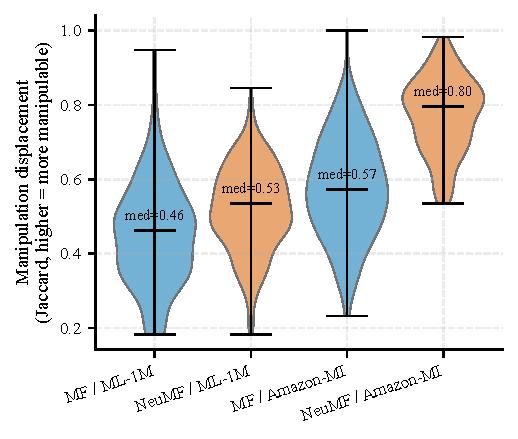
\includegraphics[width=\columnwidth]{fig2_manipulation_resistance.pdf}
    \caption{Manipulation displacement (Jaccard) across model--dataset combinations. NeuMF distributions are centered well above MF's structural floor, driven by cross-user coupling through shared embeddings.}
    \label{fig:manipulation}
\end{figure}

\subsection{Reachability Under Conservative Budgets}

Only 12.4\% of users (99/800) achieve any reachability success within budget-20 (Figure~\ref{fig:reachability}). Among reachable users, NeuMF requires fewer rating changes (mean 8.87) than MF (mean 18.93), suggesting that neural architectures create more traversable recommendation paths---but for a much smaller fraction of users (5.5\% NeuMF vs.\ 25.0\% MF on ML-1M). The high unreachability rate is not a limitation but a finding: it demonstrates that reachability cost is a stringent metric separating truly manipulable paths from structurally rigid ones. Per-combo unreachable fractions: MF/ML-1M 75.0\%, NeuMF/ML-1M 95.5\%, MF/Amazon-MI 83.0\%, NeuMF/Amazon-MI 97.0\%.

\begin{figure}[t]
    \centering
    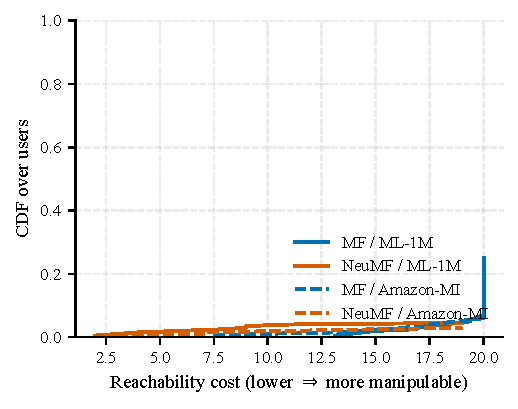
\includegraphics[width=\columnwidth]{fig1_reachability_cdf.pdf}
    \caption{CDF of reachability cost (finite-cost users only). 12.4\% of users are reachable within budget-20; NeuMF achieves lower cost (mean 8.87 flips) than MF (mean 18.93) among reachable users, but reaches far fewer users overall.}
    \label{fig:reachability}
\end{figure}

\subsection{Autonomy Asymmetry}

Users with AAI $> 1$---where adversary influence exceeds self-influence---are concentrated in MF/ML-1M (13.0\% of users; Figure~\ref{fig:aai}). Counterintuitively, NeuMF shows fewer AAI $> 1$ users (3.0\% on ML-1M, 1.0\% on Amazon-MI) despite higher absolute manipulation. This is because NeuMF's cross-user coupling also amplifies self-influence: when a user's own rating changes trigger shared-parameter updates, those updates propagate back to the user's own scores. The geometry of the scatter plot (Figure~\ref{fig:aai}) reveals that MF users cluster along the low-external, high-self axis, while NeuMF pushes users into higher-external territory but with proportionally higher self-influence.

\begin{figure*}[t]
    \centering
    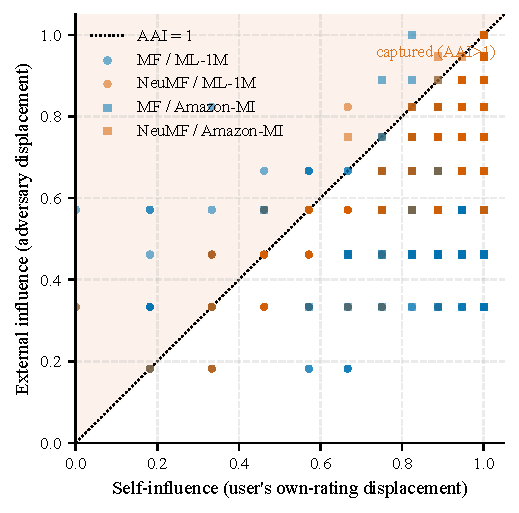
\includegraphics[width=\textwidth]{fig3_aai_scatter.pdf}
    \caption{Self-influence vs.\ external (adversary) influence per user. Points above the $y = x$ diagonal have AAI $> 1$ (adversary controls more than user). The shaded region marks causal capture. MF/ML-1M: 13.0\% above diagonal; NeuMF/Amazon-MI: 1.0\%.}
    \label{fig:aai}
\end{figure*}

\subsection{ODR Across Architectures and Datasets}

Figure~\ref{fig:odr} shows ODR across all combinations. NeuMF's deception rate exceeds MF's on both datasets (ML-1M: 90.4\% vs.\ 68.3\%; Amazon-MI: 93.9\% vs.\ 88.0\%). The observational baselines (Table~\ref{tab:odr-breakdown}) confirm that NeuMF produces higher diversity (ILD: 0.819--0.999 vs.\ 0.733--0.983) and higher volatility (0.579--0.706 vs.\ 0.128--0.359), which \emph{should} signal greater user autonomy---yet the causal metrics reveal the opposite. This is the core finding: \textbf{deeper architectures with cross-user parameter sharing trap more users while looking observationally benign}.

\begin{figure*}[t]
    \centering
    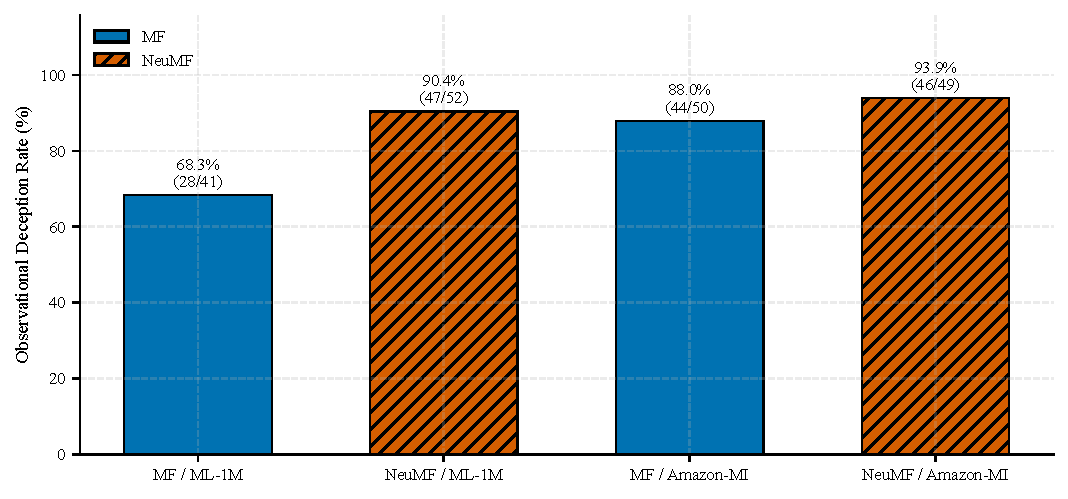
\includegraphics[width=\textwidth]{fig4_odr_comparison.pdf}
    \caption{Observational Deception Rate across model--dataset combinations. ODR measures the fraction of observationally autonomous users who are causally trapped. NeuMF consistently exceeds MF, reaching 93.9\% on Amazon-MI.}
    \label{fig:odr}
\end{figure*}


%% ═════════════════════════════════════════════════════════════════════
\section{Discussion}
\label{sec:discussion}
%% ═════════════════════════════════════════════════════════════════════

\paragraph{Implications for auditing practice.}
Our results challenge the common assumption that diversity and volatility metrics suffice for autonomy auditing. Under the EU Digital Services Act~\cite{eu_dsa2022}, platforms must assess ``systemic risks'' including effects on fundamental rights. If auditors rely exclusively on observational metrics, they risk certifying systems as autonomy-respecting when 68--94\% of apparently autonomous users are in fact causally trapped. CausalLens provides the complementary causal layer that regulation implicitly requires.

\paragraph{The architecture matters.}
The consistent gap between MF and NeuMF across all metrics demonstrates that model architecture is not merely an implementation detail for auditing purposes. Shared parameters create coupling channels invisible to observational metrics. As recommender systems adopt increasingly complex architectures (transformers, graph neural networks), causal auditing becomes more---not less---necessary.

\paragraph{Limitations.}
Our reachability budget ($B = 20$) is conservative; higher budgets would likely increase reachability rates. The two architectures (MF, NeuMF) are relatively simple compared to production systems. ODR thresholds at population medians are a natural choice but not the only valid one. CausalLens currently requires model-level access (white-box or retrain-capable); pure API-only auditing with no retrain capability remains an open challenge.


%% ═════════════════════════════════════════════════════════════════════
\section{Conclusion}
\label{sec:conclusion}
%% ═════════════════════════════════════════════════════════════════════

We presented CausalLens, an open-source toolkit that operationalizes causal autonomy auditing for recommender systems. Across 800 user evaluations on two architectures and two datasets, we demonstrated that 68--94\% of observationally autonomous users are causally trapped---a finding invisible to standard diversity and volatility metrics. Neural architectures with shared parameters amplify this deception: NeuMF produces higher observational diversity while creating stronger cross-user manipulation channels. CausalLens is publicly available and reproduces our full experimental pipeline on a single laptop.

%% ── acknowledgments ─────────────────────────────────────────────────
\begin{acks}
We thank the anonymous reviewers for their feedback. This work was supported by the University of Calgary.
\end{acks}

%% ── references ──────────────────────────────────────────────────────
\bibliographystyle{ACM-Reference-Format}
\bibliography{references}

\end{document}
